\documentclass[11pt,a4paper]{article}

\usepackage[a4paper, top=1in, bottom=1in, left=1in, right=1in]{geometry}

\usepackage{tikz}
\usepackage{amssymb}
\usepackage{amsmath}
\usepackage{graphicx}
\usepackage{float}

\setlength{\parskip}{2pt}

\begin{document}

    %\input{frontispiece.tex}
    
    \begin{center}
        \Huge Congruence Closure Solver

        \LARGE Project Report 2024-2025

        \Large {Luca Panariello VR518122}
    \end{center}

    \vspace{0.5em}

    \section{Introduction}

    The project consists of creating a \textbf{solver} for the satisfiability of formulas belonging to three different theories: the theory of equality with free symbols, non-empty possibly cyclic lists, and arrays without extensionality.

    The solver uses the \textbf{Congruence Closure Algorithm} on a DAG and has three possible variations or heuristics that can be chosen optionally:
    \textbf{Non-recursive} \texttt{FIND} function, \textbf{Heuristic} \texttt{UNION}, \textbf{Forbidden Set} use.

    This project is written in \textbf{Java} language, used due to many build-in optimized datas stucture implemented and easy testing enviroment. 

    Along the solver, there is a \textbf{generator} for the creation of a synthetic set of literals customizable by the user (under a cert extent), and a \textbf{parser} for a limited set of \textbf{QF\_UF SMT-LIB} files.

    \section{Project Folder}
    The project folder is organized in the following way:
    \begin{itemize}
        \item \textbf{analyzed}: this folder contains output files used in table and graphic.
        \item \textbf{generator}: this folder contains the properties files used by \texttt{Generator}
        \item \textbf{input}: this folder contains the txt files that have the formula or set of literals to be checked, those files use the basic syntax of the solver.
        \item \textbf{output}: this folder contains the result submitted in the input folder.
        \item \textbf{smtlib\_input}: this folder contains the .smt2 files from SMT-LIB without edit.
    \end{itemize}

    The other folders containain java files and compiled class files.

    The main class is \texttt{Congruence Closure Solver} which acts as \textbf{central manager} and is responsible for reading the name file given in input (that has to be in \texttt{input}, \texttt{generator}, \texttt{smtlib\_input} folder based on the type of file), the options and retrieves the formula using a \texttt{FormulaReader}. The formula will be passed to a \textbf{parser} and then to the \textbf{algorithm}.

    \section{Input}

    The program accepts both a \textbf{set of literals} delimited by \texttt{;} and a formula with \textbf{logical connectives}.

    It is also possible to submit a generator file with \texttt{.properties} extension to create a customizable set of literals, with \textbf{random} mechanisms.

    Or to submit directly a \texttt{.smt2} file from QF\_UF SMT-LIB, not all the files are compatible since the SMT-LIB language is very complex.

    More info about the syntax is available in the \texttt{README} file.

    \section{Parsing}

    The retrieved formula is submitted by a chain of parsers:
    \begin{enumerate}
        \item \texttt{DNFParser}: after dropping the \textbf{existential} quantifiers and the \textbf{universal} quantifiers, parse the input formula and cast it in a \texttt{DNFTree}, a $n$-tree where the nodes are \textbf{logical connectives} or \textbf{predicates}, and the edge are the scope of the logical connectives.
        
        (More info about the precedence used in in the \texttt{README} file)
        
        For example, the formula $[\lnot A \lor [B \implies C] ] \iff [\lnot[ D \land E]]$ is encoded as:

        \begin{center}
            \begin{tikzpicture}[
                level distance=0.7cm,
                level 1/.style={sibling distance=5cm},
                level 2/.style={sibling distance=2.5cm},
                level 3/.style={sibling distance=1.5cm}
            ]
                \node[] (root) {$\iff$}
                    child {node[] {$\lor$} 
                        child {node[] {$\lnot$}
                            child{
                                node [] {$A$}
                            }
                            edge from parent node[above left] {}
                        }
                        child {node[] {$\implies$} 
                            child {node[] {$B$} 
                                edge from parent node[above left] {}}
                            child {node[] {$C$} 
                                edge from parent node[above right] {}}
                            edge from parent node[above] {}
                        }
                        edge from parent node[above left] {}
                    }
                    child {node[] {$\lnot$} 
                        child {node[] {$\land$} 
                            child {node[] {D} 
                                edge from parent node[above left] {}}
                            child {node[] {E} 
                                edge from parent node[above right] {}}
                            edge from parent node[above left] {}
                        }
                        edge from parent node[above right] {}
                    };
            \end{tikzpicture}
        \end{center}

        \item \texttt{LogicParser}: use the \texttt{DNFTrasformer} handle a chain of transformation that reduces the \texttt{DNFTree} to a tree with an \texttt{OR} root that has only have \texttt{AND} children, which will have only predicate children (already negated if is the case), which will be the \textbf{leaves}.

        Then cast the leaves into an \texttt{ArrayList<String>} which will represent the list of \textbf{cubes} to solve one at a time.

        Another task that the \texttt{LogicParser} performs is the \textbf{splitting} required upon receiving a formula that contains an instance of \texttt{select(score($\dots$))}, the parser checks the occurrence and splits the formula in the two versions since it has handled a list of cubes (\texttt{OR}) than the parser removed the split cube, and enqueue the new ones, ready to be checked at the end, and performing the operation again if necessary.

        \item \texttt{Term Parser}: it receives a set of clauses one per time, and converts the literals in \textbf{nodes}.

        It handles both predicate $P(a)$ or $\lnot P(a)$ and converts them inequalities using a true constant, that the user cannot insert in the input: \texttt{P(a) = °} or \texttt{P(a) != °}.

        Then it splits each (dis)equality and makes a \texttt{Node} object for each of them with an associated (\texttt{int}) \texttt{id}, each node is contained in an \texttt{HashMap<Integer,Node>} for easy access, while the pair of id of term \texttt{L} associated with a (dis)equality are stored in two \texttt{ArrayList<Integer[]>}, in this case \texttt{L[0]} is the left term while \texttt{L[1]} is the right term. 
        
        The parser also updates the \textbf{Forbidden Sets} of the nodes even if they will not be used if the option is not toggled.

        While processing the terms the parser recognizes the presence of a reserved name, if the given formula is in one of the three compatible \textbf{theories}. Since the parser can not handle a combination of theories, if two reserved names from the theory of \textbf{list} and \textbf{array} are detected, then the parser will consider the formula in the theory of \textbf{equality}, using the reserved name function as free symbols.
        
        The last task is address to do, is the \textbf{transformation} required by the list of theory, such \texttt{~atom(a)} into \texttt{cons(a\_1,a\_2) = a}, applying \textbf{projection atoms} and adding disequalities such as: \texttt{cons(x,y) != atom(z)} for each \texttt{x,y,z} occurrence. 

    \end{enumerate}

    \section{Congruence Closure Algorithm}

    After all parsing steps, for each cube, the \texttt{TermParser} forward the map of \texttt{Node} objects and the \texttt{ArrayList<Integer[]>} of (dis)equalities to the \texttt{CongruenceClosureAlgorithm} implemented with a \texttt{CongruenceClosureDAG}; this data structure along with \texttt{Node} are implemented following the definition in Bradley, Manna, et al. \cite{calculusOfComputation}.

    The main task of \texttt{CongruenceClosureAlgorithm} is to instruct \texttt{CongruenceClosureDAG} to \texttt{MERGE} all the nodes in the equalities list, once there are no more nodes to merge, checks that the pair of id in the disequalities list is not in the same \textbf{ccpar set (implemented as a \texttt{HashSet<Integer>})}, and return a \texttt{bool} that indicates the satisfiability.

    If the \textbf{Forbidden Set} option is enabled, then the \texttt{CongruenceClosureDAG} will prevent the \texttt{MERGE} of two representatives of disequalities, and return to the algorithm the conflict, which will return unsat. If no conflicts are found, then \texttt{CongruenceClosureAlgorithm} will skip the checking disequalities part.

    If the \textbf{Heuristic Union} or the \textbf{Recursive Find} options are enabled then the \texttt{EUR\_UNION} and \texttt{REC\_FIND} version will be used as described in Detlefs, et al. \cite{simplify}.

    \section{Output}

    The result will be written in a txt file in the output with the same name as the file in the input one.
    If the \textbf{verbose} \texttt{"v"} option is enabled, then all the steps of the \texttt{CongruenceClosureDAG} will be written, it is advisable to not enable this option is for long formula or in CNF since the transformation in DNF is very prolific.
    
    At the end of the file will be written the result and the time elapsed for the solving, which do not take into account the time in DNF transformation.

    \section{Sintetic Generator}

    Along the solver is present a \texttt{Generator} which will write a set of literals based on the user's \textbf{choices}.

    The user can choose the \textbf{signature} (constant, functions and predicate), the max \textbf{arity} for functions and predicates, the max \textbf{depth} of a function or predicate, the number of \textbf{cubes} to generate, the \textbf{probabilities} of the presence of constants, function or predicates, and the optionally the \textbf{seed}, so that the randomly generated formula can be replicated, with same parameters.

    It is advised to restrain depth and artity to 10, and cubes to 100, since the Java memory cannot handle too many \texttt{Node} structures.

    The generator will place the synthetic list of literals in a txt file in the input folder with the same name as the properties file, concatenated with the seed. 

    The execution of the solver is automatic after the submission of the file name.

    \section{SMT-LIB}

    Since the \textbf{SMT-LIB} language features a lot of definition and syntax, only a restricted subset of formulas of the QF\_UF have been made compatible with the \texttt{SMTLIBParser} in particular the formulas present in \texttt{eq\_diamond} from SMT Workshop 2005.

    In these files are present only an \texttt{assert} check for a formula written in this form:

    \begin{equation}
        \bigwedge_i \left(\bigvee_j x_{i,j} \simeq y_{i,j} \land z_{i,j} \simeq w_{i,j} \right) 
        \land u \not\simeq v \quad u,v \in \{x_{i,j}, y_{i,j}, z_{i,j}, w_{i,j} \mid \forall i,j\}
    \end{equation} 
    The \textbf{length} of the formula is determined by the number of equations, (eq\_diamond4 is larger than eq\_diamond2) and the result of all formulas are UNSAT, so are been used to test the heuristics implemented in this project.

    As for the \texttt{Generator}, the smt2 files have to be placed in the \textbf{smtlib\_input} and an equivalent parsed formula with the project syntex, will be written in a txt file in the input folder with the same name. 

    The execution of the solver is automatic after the submission of the file name.

    Since the DNF transformation is not optimized, it is not advisable to run eq\_diamond15 or larger.

    \section{Performance Analysis}

    The solver works with all the files located in \texttt{input} folder, but some of them have 
    been analyzed using different option, these results can be found in \texttt{analyzed} folder
    and used to create the following table and graphic.

    \newcommand{\selected}{X}

    \begin{table}[ht]
        \centering
        \begin{tabular}{|l|c|c|c|c|c|c|}
        \hline
            \textbf{Name}           & \textbf{Recursive}    & \textbf{H-Union}  & \textbf{Forbidden}    & \textbf{Time} & \textbf{Result} \\ \hline
            ArrayBM9.8d\_r          & \selected             &                   &                       & 0.000s        & UNSAT \\ \hline
            ArrayBM9.8d\_re         & \selected             & \selected         &                       & 0.001s        & UNSAT \\ \hline
            ArrayBM9.8d\_rf         & \selected             &                   & \selected             & 0.000s        & UNSAT \\ \hline
            EqMB1.8.txt             &                       &                   &                       & 0.002s        & SAT   \\ \hline  
            EqMB1.8\_r.txt          & \selected             &                   &                       & 0.003s        & SAT   \\ \hline  
            EqMB1.8\_e.txt          &                       & \selected         &                       & 0.002s        & SAT   \\ \hline  
            EqMB1.8\_f.txt          &                       &                   & \selected             & 0.002s        & SAT   \\ \hline  
            ListBM9.6b              &                       &                   &                       & 0.011s        & UNSAT \\ \hline               
            ListBM9.6b\_ref.txt     & \selected             & \selected         & \selected             & 0.009s        & UNSAT \\ \hline
            eq\_diamond10\_r        & \selected             &                   &                       & 0.613s        & UNSAT \\ \hline
            eq\_diamond10\_ef       &                       & \selected         & \selected             & 0.316s        & UNSAT \\ \hline
            eq\_diamond12\_r        & \selected             &                   &                       & 6.246s        & UNSAT \\ \hline
            eq\_diamond12\_ef       &                       & \selected         & \selected             & 6.143s        & UNSAT \\ \hline
            eq\_diamond14\_r.smt2   & \selected             &                   &                       & 91.30s        & UNSAT \\ \hline
            eq\_diamond14\_ef.smt2  &                       & \selected         & \selected             & 89.49s        & UNSAT \\ \hline
            eq\_diamond14.smt2      &                       &                   &                       & 88.06s        & UNSAT \\ \hline
            eq\_diamond14\_f.smt2   &                       &                   & \selected             & 87.10s        & UNSAT \\ \hline
            
            GEN100.properties       &                       &                   &                       & 0.074s        & SAT   \\ \hline
            GEN100\_r.properties    & \selected             &                   &                       & 0.067s        & SAT   \\ \hline
            GEN100\_e.properties    &                       & \selected         &                       & 0.076s        & SAT   \\ \hline  
            GEN100\_f.properties    &                       &                   & \selected             & 0.080s        & SAT   \\ \hline
            GEN100\_re.properties   & \selected             & \selected         &                       & 0.071s        & SAT   \\ \hline
            GEN100\_rf.properties   & \selected             &                   & \selected             & 0.070s        & SAT   \\ \hline
            GEN100\_ef.properties   &                       & \selected         & \selected             & 0.077s        & SAT   \\ \hline
            GEN100\_ref.properties  & \selected             & \selected         & \selected             & 0.072s        & SAT   \\ \hline
        \end{tabular}
        \caption{Test Results Table}
    \end{table}
    For short formulas, the different options have no significant impact.

    However, for medium-sized formulas, the recursive version of \texttt{FIND} appears to boost performance. The idea behind the \textbf{Non-Recursive} approach is to reduce the recursive calls of \texttt{FIND} at the cost of updating the representatives of all nodes associated with a representative node that is not chosen during the \texttt{MERGE}. This will be referred to as the \textbf{Non-Recursive Burden}.
    
    For large formulas, the \textbf{Forbidden Set} significantly improves the speed of detecting conflicts in most of the cases. However, using \textbf{Heuristic Union} slows down the process. This could be due to the implementation of the heuristic, as the representative node is chosen based on the larger ccpar set. Each time there is a \texttt{MERGE}, there may be a potential sub-\texttt{MERGE} between different but congruent ccpar elements of the two terms. If both terms have large ccpar sets, this increases the resolution time. This phenomenon will be referred to as the \textbf{H-Union Burden}.

    The elapsed times vary depending on whether only recursive \texttt{FIND} (without heuristics) is used or all heuristics are applied, based on the formula size. The following graphic illustrates which formula sizes are better served by these approaches.

    \begin{figure}[H]
        \centering
        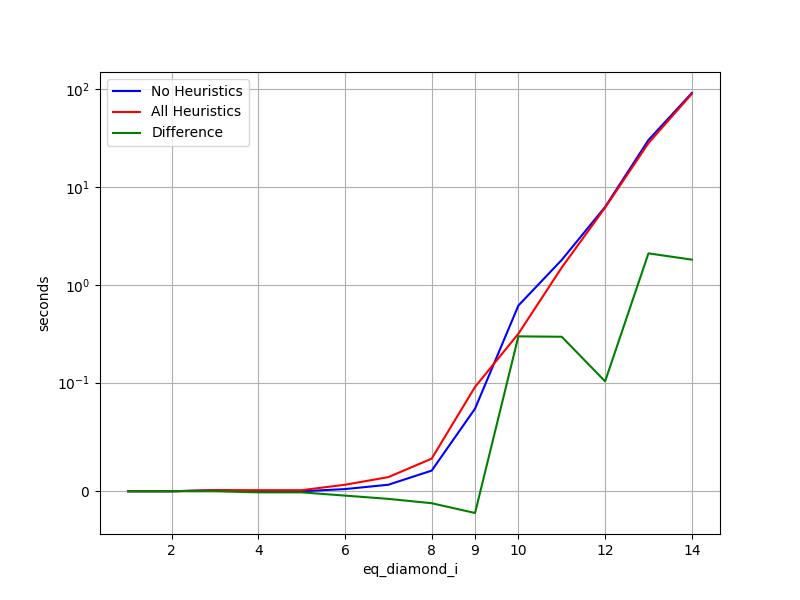
\includegraphics[width=10cm]{graphic.png}
        \caption{Comparison of Performance With and Without Heuristics}
        \label{fig:graphic}
    \end{figure}

    As the graphic shows, the heuristics become helpful after \texttt{eq\_diamond9.smt2}, as indicated by the green line (Heuristic Time - No Heuristic Time).

    Between \texttt{eq\_diamond5.smt2} and \texttt{eq\_diamond9.smt2}, the \textbf{Non-Recursive Burden} and \textbf{H-Union Burden} are heavier. 

    The algorithm spends significant time updating the representatives, which happens frequently due to the heuristics. This is not justifiable since the formulas are not large. A more distributed ccpar set size, without requiring checks from all nodes for representative changes, could be beneficial.

    Meanwhile, the \textbf{Forbidden Set} does not seem to help much, as passing all the IDs in the set between representatives and non-representatives can be expensive. Another reason could be that the formula size is insufficient to justify this overhead.

    For \texttt{eq\_diamond9.smt2} and larger formulas, the difference between using heuristics and not is noticeable. With many literals to check, recursion and distribution of large ccpar sizes can be more expensive than the \textbf{Non-Recursive Burden} and \textbf{H-Union Burden}.

    %Perhaps with the introduction of parallelism and a better implementation of the DNF transformation, it might be possible to handle larger formulas within a manageable time, enabling further investigation to confirm or refute this conjecture.

    \bibliographystyle{unsrt}
    \bibliography{bibliography}    

\end{document}